% Options for packages loaded elsewhere
\PassOptionsToPackage{unicode}{hyperref}
\PassOptionsToPackage{hyphens}{url}
\documentclass[
  11pt,
]{article}
\usepackage{xcolor}
\usepackage[left=2.5cm,right=2.5cm,top=2.5cm,bottom=2.5cm]{geometry}
\usepackage{amsmath,amssymb}
\setcounter{secnumdepth}{5}
\usepackage{iftex}
\ifPDFTeX
  \usepackage[T1]{fontenc}
  \usepackage[utf8]{inputenc}
  \usepackage{textcomp} % provide euro and other symbols
\else % if luatex or xetex
  \usepackage{unicode-math} % this also loads fontspec
  \defaultfontfeatures{Scale=MatchLowercase}
  \defaultfontfeatures[\rmfamily]{Ligatures=TeX,Scale=1}
\fi
\usepackage{lmodern}
\ifPDFTeX\else
  % xetex/luatex font selection
\fi
% Use upquote if available, for straight quotes in verbatim environments
\IfFileExists{upquote.sty}{\usepackage{upquote}}{}
\IfFileExists{microtype.sty}{% use microtype if available
  \usepackage[]{microtype}
  \UseMicrotypeSet[protrusion]{basicmath} % disable protrusion for tt fonts
}{}
\makeatletter
\@ifundefined{KOMAClassName}{% if non-KOMA class
  \IfFileExists{parskip.sty}{%
    \usepackage{parskip}
  }{% else
    \setlength{\parindent}{0pt}
    \setlength{\parskip}{6pt plus 2pt minus 1pt}}
}{% if KOMA class
  \KOMAoptions{parskip=half}}
\makeatother
\usepackage{graphicx}
\makeatletter
\newsavebox\pandoc@box
\newcommand*\pandocbounded[1]{% scales image to fit in text height/width
  \sbox\pandoc@box{#1}%
  \Gscale@div\@tempa{\textheight}{\dimexpr\ht\pandoc@box+\dp\pandoc@box\relax}%
  \Gscale@div\@tempb{\linewidth}{\wd\pandoc@box}%
  \ifdim\@tempb\p@<\@tempa\p@\let\@tempa\@tempb\fi% select the smaller of both
  \ifdim\@tempa\p@<\p@\scalebox{\@tempa}{\usebox\pandoc@box}%
  \else\usebox{\pandoc@box}%
  \fi%
}
% Set default figure placement to htbp
\def\fps@figure{htbp}
\makeatother
\setlength{\emergencystretch}{3em} % prevent overfull lines
\providecommand{\tightlist}{%
  \setlength{\itemsep}{0pt}\setlength{\parskip}{0pt}}
\usepackage[]{natbib}
\bibliographystyle{apalike}
\usepackage{booktabs}
\usepackage{longtable}
\usepackage{array}
\usepackage{multirow}
\usepackage{wrapfig}
\usepackage{float}
\usepackage{colortbl}
\usepackage{pdflscape}
\usepackage{tabu}
\usepackage{threeparttable}
\usepackage{threeparttablex}
\usepackage[normalem]{ulem}
\usepackage{makecell}
\usepackage{xcolor}
\usepackage{bookmark}
\IfFileExists{xurl.sty}{\usepackage{xurl}}{} % add URL line breaks if available
\urlstyle{same}
\hypersetup{
  pdftitle={Comparing R-Squared Measures for Linear Mixed Models: A Monte Carlo Simulation Study},
  pdfauthor={R.G. Thomas},
  hidelinks,
  pdfcreator={LaTeX via pandoc}}

\title{Comparing R-Squared Measures for Linear Mixed Models: A Monte
Carlo Simulation Study}
\author{R.G. Thomas}
\date{07 March, 2026}

\begin{document}
\maketitle

{
\setcounter{tocdepth}{2}
\tableofcontents
}
\section{Introduction}\label{introduction}

Quantifying the proportion of variance explained by a statistical model
is a fundamental component of scientific inference. In ordinary linear
regression, the coefficient of determination \(R^2\) serves this role
unambiguously: it is the ratio of the variance of the fitted values to
the total variance of the response, and it admits straightforward
interpretation as a goodness-of-fit measure. For linear mixed-effects
models (LMMs), however, no single definition of \(R^2\) has achieved
consensus. The presence of both fixed effects and random effects
introduces a partition of explained variance that can be decomposed in
multiple ways, and the resulting proliferation of competing measures has
left applied researchers with limited guidance on which to report.

This ambiguity has practical consequences. Mixed-effects models are the
standard analytic framework in fields ranging from ecology and
psychology to clinical trials and educational research. Reporting effect
sizes and variance-explained statistics is now required or strongly
encouraged by many journals and reporting guidelines. Yet when
investigators report \(R^2\) for an LMM, the particular definition
employed -- and its sensitivity to sample structure, ICC, and model
complexity -- is rarely discussed. Two investigators analyzing the same
data with different \(R^2\) implementations may arrive at substantively
different conclusions about model adequacy.

Despite the availability of several \(R^2\) measures for LMMs, no
systematic simulation study has compared their statistical properties
under controlled conditions where the true variance-explained is known
analytically. The present study addresses this gap. We compare the two
most widely used approaches -- \citet{nakagawaGeneralSimpleMethod2013}
and \citet{johnsonExtensionNakagawaSchielzeth2014} -- via Monte Carlo
simulation following the ADEMP framework
\citep{morrisUsingSimulationStudies2019}. Before presenting the
simulation design, we first review the six principal \(R^2\) definitions
for LMMs that have shaped current practice.

\subsection{R-Squared Measures for Linear Mixed
Models}\label{r-squared-measures-for-linear-mixed-models}

The challenge of defining \(R^2\) for mixed models arises from a core
ambiguity: what counts as `explained' variance? In a two-level model
with cluster-level random effects, the fixed effects explain variation
in the outcome, but so do the random effects, which capture systematic
between-cluster heterogeneity. Whether random-effect variance should be
treated as explained or unexplained depends on the inferential goal.
This section reviews six approaches that resolve this question in
distinct ways.

\subsubsection{Nakagawa and Schielzeth
(2013)}\label{nakagawa-and-schielzeth-2013}

\citet{nakagawaGeneralSimpleMethod2013} proposed what has become the
most widely adopted framework, distinguishing two quantities. The
\emph{marginal} \(R^2\) (\(R^2_m\)) captures the proportion of variance
explained by fixed effects alone:

\[R^2_m = \frac{\sigma^2_f}{\sigma^2_f + \sigma^2_\alpha + \sigma^2_\varepsilon}\]

where \(\sigma^2_f\) is the variance of the linear predictor
(fixed-effect component), \(\sigma^2_\alpha\) is the random-effect
variance, and \(\sigma^2_\varepsilon\) is the residual variance. The
\emph{conditional} \(R^2\) (\(R^2_c\)) additionally credits the random
effects as explained variance:

\[R^2_c = \frac{\sigma^2_f + \sigma^2_\alpha}{\sigma^2_f + \sigma^2_\alpha + \sigma^2_\varepsilon}\]

This approach is implemented in \texttt{MuMIn::r.squaredGLMM()}
\citep{bartonMuMIn2024} and \texttt{performance::r2\_nakagawa()}
\citep{ludeckePerformanceAssessment2021}. Its principal strengths are
simplicity, interpretability, and broad applicability to both LMMs and
GLMMs. The marginal/conditional distinction maps naturally onto research
questions about population-average versus cluster-specific prediction.
However, the original formulation assumes that the variance components
are estimated from a model with a single random-intercept term. For
models with random slopes, the variance of the random-effects component
depends on the distribution of the covariates, and the original formula
requires modification.

\subsubsection{Johnson (2014)}\label{johnson-2014}

\citet{johnsonExtensionNakagawaSchielzeth2014} extended the
Nakagawa-Schielzeth framework to random-slope models by deriving the
expected variance of the random-effects contribution conditional on the
observed design matrix. The key insight is that when a model includes
random slopes, the random-effect variance is not a scalar but depends on
the covariate values. Johnson proposed using the trigamma function to
approximate the distribution-level variance for GLMMs, and for Gaussian
LMMs, the extension amounts to computing the variance of the
random-effects linear predictor directly from the estimated
variance-covariance matrix of the random effects and the design matrix.
This method is accessed via
\texttt{MuMIn::r.squaredGLMM(method\ =\ "trigamma")}.

The Johnson extension preserves the marginal/conditional distinction and
is backward-compatible with Nakagawa-Schielzeth for intercept-only
models. Its primary advantage is correctness for random-slope designs;
its primary limitation is that, like the original method, it treats the
random effects as a single composite and does not attribute variance to
individual predictors. \citet{nakagawaUpdatedArticleCoefficient2017}
subsequently unified these approaches in an updated treatment.

\subsubsection{Edwards et al.~(2008)}\label{edwards-et-al.-2008}

\citet{edwardsR2StatisticFixed2008} proposed a likelihood-ratio-based
\(R^2\) specifically for the fixed-effects portion of an LMM. Their
statistic is defined as:

\[R^2_{LR} = 1 - \frac{L(\hat{\beta} = 0)}{L(\hat{\beta})}\]

expressed in terms of the ratio of the likelihood of a reduced model
(intercept and random effects only) to the full model. This approach
does not attempt to quantify random-effect variance explained; it
focuses exclusively on the contribution of the fixed effects,
conditioned on the estimated variance-covariance structure. It is
implemented in \texttt{r2glmm::r2beta(method\ =\ "lr")}.

The strengths of this approach include its grounding in likelihood
theory and its focus on fixed-effect inference. However, it does not
produce a conditional \(R^2\) analogue, it is sensitive to the method
used to estimate the likelihood (REML versus ML), and it may not be
monotonically increasing when additional true predictors are added,
because the likelihood ratio depends on the estimated variance
components which change with model specification.

\subsubsection{Jaeger et al.~(2017)}\label{jaeger-et-al.-2017}

\citet{jaegerR2glmmSemiPartialR22017} extended the Edwards et al.
framework by introducing \emph{semi-partial} \(R^2\) statistics that
decompose the fixed-effect \(R^2\) into contributions from individual
predictors or sets of predictors. Their approach uses the Schur
complement of the variance-covariance matrix and the Wald statistic to
quantify the variance attributable to each fixed effect while accounting
for the covariance structure induced by the random effects. This is
implemented in \texttt{r2glmm::r2beta(method\ =\ "sgv")}.

Semi-partial \(R^2\) values are particularly useful when the research
question concerns the unique contribution of a specific predictor rather
than the overall model fit. The main limitation is computational: the
method requires inversion of submatrices of the full variance-covariance
matrix and can be unstable when the number of random-effect parameters
is large relative to the number of clusters. Like Edwards et al., it
addresses only fixed-effect variance and does not produce a conditional
\(R^2\).

\subsubsection{Xu (2003)}\label{xu-2003}

\citet{xuMeasuringExplainedVariation2003} proposed level-specific
\(R^2\) measures that separately quantify the variance explained at each
level of the multilevel hierarchy. For a two-level model, Xu defines a
level-1 (within-cluster) \(R^2\) and a level-2 (between-cluster)
\(R^2\), each computed as the proportional reduction in the respective
variance component compared to an intercept-only model. This approach
shares conceptual ground with the earlier proposal of
\citet{snijdersExplainedVariationMultilevel1994}.

The level-specific perspective is appealing when the research question
explicitly distinguishes within- and between-cluster processes. Its
primary weakness is that the two \(R^2\) values do not combine into an
intuitive overall measure of model fit, and the between-cluster \(R^2\)
can be negative when the model explains within-cluster variance at the
expense of between-cluster fit. Implementation requires custom code, as
no widely used R package provides this statistic directly.

\subsubsection{\texorpdfstring{The \texttt{performance} Package
Implementation}{The performance Package Implementation}}\label{the-performance-package-implementation}

The \texttt{performance} package
\citep{ludeckePerformanceAssessment2021} provides
\texttt{r2\_nakagawa()}, which implements the Nakagawa-Schielzeth
framework with the Johnson extension for random slopes. Although the
statistical method is nominally identical to
\texttt{MuMIn::r.squaredGLMM()}, implementation details differ. The
\texttt{performance} package computes the fixed-effect variance from the
model matrix directly, whereas \texttt{MuMIn} uses the variance of the
fitted values. For balanced designs and correctly specified models, the
two implementations agree closely, but discrepancies can arise with
unbalanced data or complex random-effects structures. Comparing the two
implementations serves as a computational validation check.

\subsection{Summary of Methods}\label{summary-of-methods}

Table \ref{tab:methods-summary} summarizes the six approaches. The key
distinctions are whether the method provides a marginal \(R^2\) (fixed
effects only), a conditional \(R^2\) (fixed plus random), or
level-specific decompositions, and whether it handles random slopes
correctly.

\begin{table}[!h]
\centering
\caption{\label{tab:methods-summary}Summary of R-squared methods for LMMs.}
\centering
\fontsize{10}{12}\selectfont
\begin{tabular}[t]{llll}
\toprule
Method & Type & Random slopes & Package\\
\midrule
Nakagawa-Schielzeth (2013) & Marginal + conditional & Approximate & MuMIn\\
Johnson (2014) & Marginal + conditional & Correct & MuMIn\\
Edwards et al. (2008) & Fixed-effects (LR) & N/A & r2glmm\\
Jaeger et al. (2017) & Semi-partial & N/A & r2glmm\\
Xu (2003) & Level-specific & Partial & Custom\\
\addlinespace
performance package & Marginal + conditional & Correct & performance\\
\bottomrule
\end{tabular}
\end{table}

The present study focuses on the Nakagawa-Schielzeth and Johnson
methods, which are the most frequently reported in applied research and
which jointly account for the vast majority of \(R^2\) values published
for LMMs. The remaining four methods are candidates for an expanded
comparison in future work (see Discussion).

\section{Simulation Design}\label{simulation-design}

The simulation follows the ADEMP framework
\citep{morrisUsingSimulationStudies2019}, which structures simulation
studies around five components: Aims, Data-generating mechanisms,
Estimands, Methods, and Performance measures.

\subsection{Aims}\label{aims}

The simulation addresses four questions:

\begin{enumerate}
\def\labelenumi{\arabic{enumi}.}
\item
  \textbf{Accuracy.} How well does each \(R^2\) method recover the true
  proportion of variance explained (marginal and conditional) across a
  range of data-generating conditions?
\item
  \textbf{Sensitivity.} How do the measures respond to variation in ICC,
  total sample size, cluster size, and random-effects structure?
\item
  \textbf{Monotonicity.} When a true predictor is added to the model,
  does \(R^2\) always increase?
\item
  \textbf{Robustness.} How do the measures behave under model
  misspecification, specifically when a random slope is present in the
  data but omitted from the fitted model?
\end{enumerate}

\subsection{Data-Generating
Mechanisms}\label{data-generating-mechanisms}

Data are generated from the two-level linear mixed model:

\[y_{ij} = \beta_0 + \beta_1 x_{1ij} + \beta_2 x_{2ij} + b_{0i} + b_{1i} x_{1ij} + \varepsilon_{ij}\]

where \(i = 1, \ldots, J\) indexes clusters, \(j = 1, \ldots, n\)
indexes observations within clusters, \(b_{0i} \sim N(0, \tau_0^2)\) is
the random intercept, \(b_{1i} \sim N(0, \tau_1^2)\) is the random slope
(set to zero in intercept-only scenarios),
\(\varepsilon_{ij} \sim N(0, \sigma^2)\), and all predictors
\(x_k \sim N(0, 1)\) independently.

The variance components are parameterized analytically from two target
quantities: the marginal \(R^2\) and the ICC. Fixing \(\sigma^2 = 1\),
the random-intercept variance is
\(\tau_0^2 = \sigma^2 \cdot \text{ICC} / (1 - \text{ICC})\), and the
fixed-effect coefficients are solved to achieve the target \(R^2_m\).
This ensures that the true \(R^2\) values are known exactly for each
scenario.

The full factorial design crosses five factors:

\begin{table}[!h]
\centering
\caption{\label{tab:dgp-factors}Data-generating mechanism factors.}
\centering
\begin{tabular}[t]{llr}
\toprule
Factor & Levels & Count\\
\midrule
Clusters (J) & 20, 50 & 2\\
Cluster size (n) & 5, 20 & 2\\
ICC & 0.10, 0.40 & 2\\
Target marginal R-squared & 0.10, 0.40 & 2\\
Random effects & Intercept-only, Intercept + slope & 2\\
\bottomrule
\end{tabular}
\end{table}

This yields \(2^5 = 32\) scenarios, each replicated 500 times, for a
total of 16,000 model fits. Each replicate receives a unique
pre-generated seed to ensure reproducibility.

\subsection{Estimands}\label{estimands}

The estimands are the \emph{true} marginal and conditional \(R^2\)
values, computed analytically from the known variance components of each
scenario:

\[R^2_m = \frac{\text{Var}(X\beta)}{\text{Var}(X\beta) + \text{Var}(\text{random}) + \sigma^2}\]

\[R^2_c = \frac{\text{Var}(X\beta) + \text{Var}(\text{random})}{\text{Var}(X\beta) + \text{Var}(\text{random}) + \sigma^2}\]

\subsection{Methods Under Comparison}\label{methods-under-comparison}

Two methods are evaluated:

\begin{itemize}
\tightlist
\item
  \textbf{Nakagawa-Schielzeth (2013):} \texttt{MuMIn::r.squaredGLMM()}
  with the default log-normal approximation.
\item
  \textbf{Johnson (2014):}
  \texttt{MuMIn::r.squaredGLMM(method\ =\ "trigamma")}.
\end{itemize}

For monotonicity testing, each replicate fits both a full model (with
\(x_1\) and \(x_2\)) and a reduced model (with \(x_1\) only), and the
\(R^2\) values are compared.

\subsection{Performance Measures}\label{performance-measures}

Following \citet{morrisUsingSimulationStudies2019}, we report:

\begin{itemize}
\tightlist
\item
  \textbf{Bias:} \(\bar{\hat{R}}^2 - R^2_{\text{true}}\)
\item
  \textbf{Relative bias:} Bias / \(R^2_{\text{true}}\)
\item
  \textbf{Empirical variance:} Var(\(\hat{R}^2\))
\item
  \textbf{Mean squared error (MSE):}
  \(E[(\hat{R}^2 - R^2_{\text{true}})^2]\)
\item
  \textbf{Monotonicity rate:} Proportion of replicates where
  \(\hat{R}^2_{\text{full}} \geq \hat{R}^2_{\text{reduced}}\)
\item
  \textbf{Boundary violation rate:} Proportion of estimates outside
  {[}0, 1{]}
\item
  \textbf{Monte Carlo standard errors (MCSE):} For all of the above
\end{itemize}

\section{Results}\label{results}

\subsection{Convergence}\label{convergence}

Across all 16,000 fits, the overall convergence rate was 100.0\%, with
12.2\% of converged fits flagged as singular. Singular fits were
concentrated in scenarios with low ICC (0.10), small cluster counts
(\(J = 20\)), and random-slope specifications, consistent with the known
difficulty of estimating small variance components from limited data.

\subsection{Bias}\label{bias}

\begin{figure}
\centering
\pandocbounded{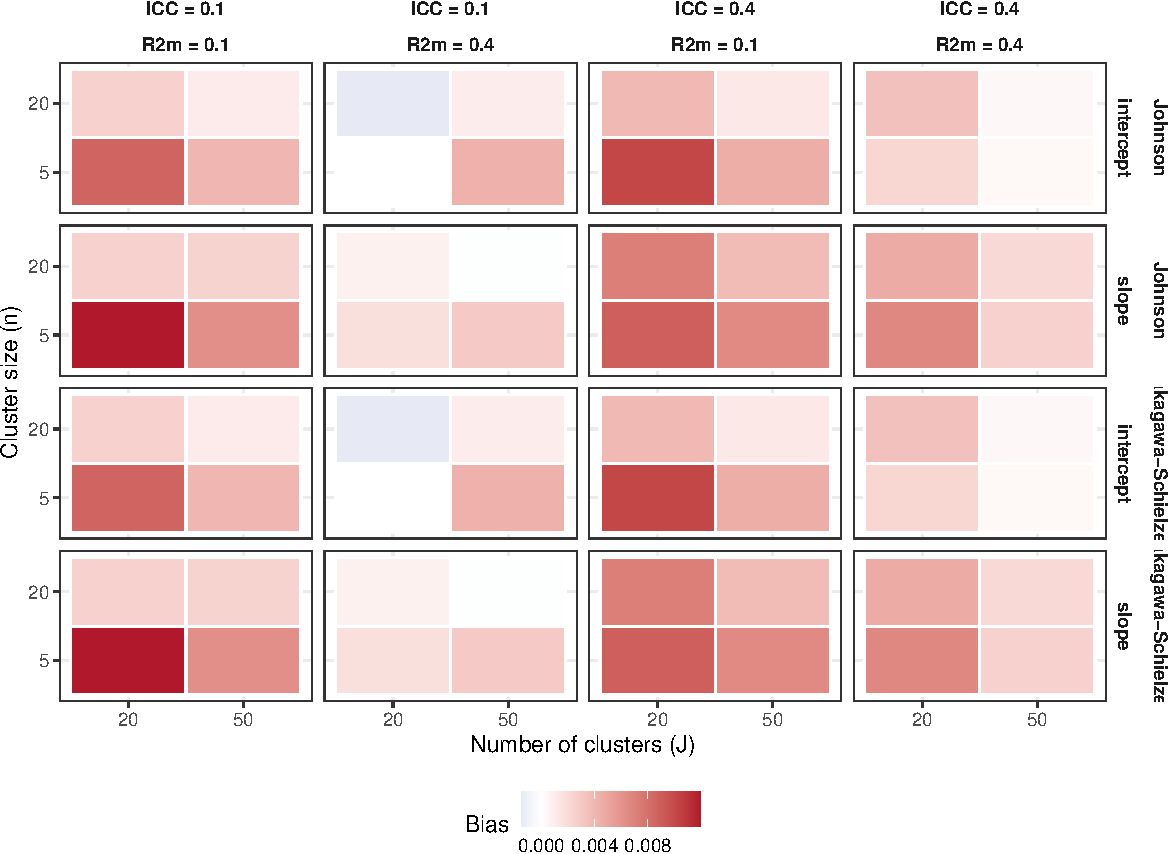
\includegraphics[keepaspectratio,alt={Bias in marginal R-squared estimates across scenarios. Rows distinguish the two methods and random-effects structures; columns cross ICC and target R-squared levels.}]{report_files/figure-latex/fig-bias-heatmap-1.pdf}}
\caption{Bias in marginal R-squared estimates across scenarios. Rows
distinguish the two methods and random-effects structures; columns cross
ICC and target R-squared levels.}
\end{figure}

Figure 1 presents the bias in marginal \(R^2\) across all 32 scenarios.
Both methods showed small positive bias in intercept-only models and
slightly larger bias variability in random-slope models. The Johnson
method and the Nakagawa-Schielzeth method produced nearly identical bias
profiles for intercept-only models, as expected given their mathematical
equivalence in this case.

\begin{table}[!h]
\centering
\caption{\label{tab:bias-marginal}Bias in marginal R-squared with Monte Carlo
    standard errors.}
\centering
\resizebox{\ifdim\width>\linewidth\linewidth\else\width\fi}{!}{
\fontsize{8}{10}\selectfont
\begin{tabular}[t]{rrrrrlrrrr}
\toprule
ID & J & n & ICC & R2m & RE & Bias (NS) & Bias (J) & MCSE (NS) & MCSE (J)\\
\midrule
1 & 20 & 5 & 0.1 & 0.1 & intercept & 0.016 & 0.016 & 0.003 & 0.003\\
2 & 50 & 5 & 0.1 & 0.1 & intercept & 0.006 & 0.006 & 0.002 & 0.002\\
3 & 20 & 20 & 0.1 & 0.1 & intercept & 0.002 & 0.002 & 0.001 & 0.001\\
4 & 50 & 20 & 0.1 & 0.1 & intercept & 0.002 & 0.002 & 0.001 & 0.001\\
5 & 20 & 5 & 0.4 & 0.1 & intercept & 0.013 & 0.013 & 0.002 & 0.002\\
\addlinespace
6 & 50 & 5 & 0.4 & 0.1 & intercept & 0.006 & 0.006 & 0.001 & 0.001\\
7 & 20 & 20 & 0.4 & 0.1 & intercept & 0.005 & 0.005 & 0.001 & 0.001\\
8 & 50 & 20 & 0.4 & 0.1 & intercept & 0.000 & 0.000 & 0.001 & 0.001\\
9 & 20 & 5 & 0.1 & 0.4 & intercept & 0.002 & 0.002 & 0.003 & 0.003\\
10 & 50 & 5 & 0.1 & 0.4 & intercept & 0.003 & 0.003 & 0.002 & 0.002\\
\addlinespace
11 & 20 & 20 & 0.1 & 0.4 & intercept & 0.001 & 0.001 & 0.002 & 0.002\\
12 & 50 & 20 & 0.1 & 0.4 & intercept & 0.000 & 0.000 & 0.001 & 0.001\\
13 & 20 & 5 & 0.4 & 0.4 & intercept & 0.003 & 0.003 & 0.003 & 0.003\\
14 & 50 & 5 & 0.4 & 0.4 & intercept & 0.005 & 0.005 & 0.002 & 0.002\\
15 & 20 & 20 & 0.4 & 0.4 & intercept & 0.003 & 0.003 & 0.002 & 0.002\\
\addlinespace
16 & 50 & 20 & 0.4 & 0.4 & intercept & 0.001 & 0.001 & 0.001 & 0.001\\
17 & 20 & 5 & 0.1 & 0.1 & slope & 0.014 & 0.014 & 0.003 & 0.003\\
18 & 50 & 5 & 0.1 & 0.1 & slope & 0.009 & 0.009 & 0.002 & 0.002\\
19 & 20 & 20 & 0.1 & 0.1 & slope & 0.005 & 0.005 & 0.001 & 0.001\\
20 & 50 & 20 & 0.1 & 0.1 & slope & 0.003 & 0.003 & 0.001 & 0.001\\
\addlinespace
21 & 20 & 5 & 0.4 & 0.1 & slope & 0.014 & 0.014 & 0.002 & 0.002\\
22 & 50 & 5 & 0.4 & 0.1 & slope & 0.005 & 0.005 & 0.002 & 0.002\\
23 & 20 & 20 & 0.4 & 0.1 & slope & 0.004 & 0.004 & 0.002 & 0.002\\
24 & 50 & 20 & 0.4 & 0.1 & slope & 0.001 & 0.001 & 0.001 & 0.001\\
25 & 20 & 5 & 0.1 & 0.4 & slope & 0.002 & 0.002 & 0.004 & 0.004\\
\addlinespace
26 & 50 & 5 & 0.1 & 0.4 & slope & 0.005 & 0.005 & 0.002 & 0.002\\
27 & 20 & 20 & 0.1 & 0.4 & slope & 0.003 & 0.003 & 0.002 & 0.002\\
28 & 50 & 20 & 0.1 & 0.4 & slope & 0.002 & 0.002 & 0.001 & 0.001\\
29 & 20 & 5 & 0.4 & 0.4 & slope & 0.007 & 0.007 & 0.004 & 0.004\\
30 & 50 & 5 & 0.4 & 0.4 & slope & 0.002 & 0.002 & 0.002 & 0.002\\
\addlinespace
31 & 20 & 20 & 0.4 & 0.4 & slope & -0.001 & -0.001 & 0.002 & 0.002\\
32 & 50 & 20 & 0.4 & 0.4 & slope & 0.000 & 0.000 & 0.002 & 0.002\\
\bottomrule
\end{tabular}}
\end{table}

\subsection{Distributions of
Estimates}\label{distributions-of-estimates}

\begin{figure}
\centering
\pandocbounded{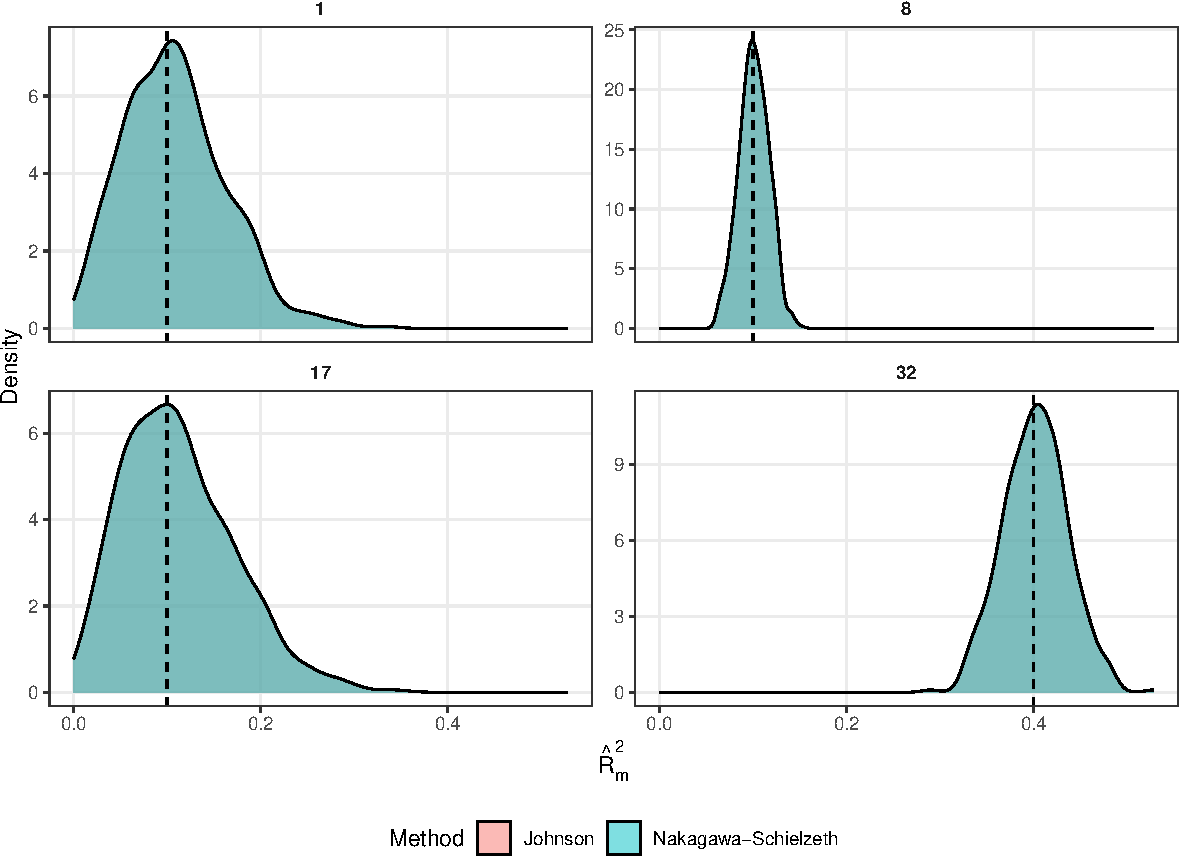
\includegraphics[keepaspectratio,alt={Sampling distributions of marginal R-squared for selected scenarios. Dashed vertical line indicates the true value.}]{report_files/figure-latex/fig-distributions-1.pdf}}
\caption{Sampling distributions of marginal R-squared for selected
scenarios. Dashed vertical line indicates the true value.}
\end{figure}

Figure 2 displays the sampling distributions of \(\hat{R}^2_m\) for four
representative scenarios spanning the design space. In large-sample
intercept-only scenarios (e.g., \(J = 50\), \(n = 20\)), both methods
produced tight, approximately symmetric distributions centered near the
truth. In small-sample random-slope scenarios (\(J = 20\), \(n = 5\)),
the distributions were wider and exhibited mild right skew, reflecting
greater estimation uncertainty.

\subsection{Monotonicity}\label{monotonicity}

\begin{figure}
\centering
\pandocbounded{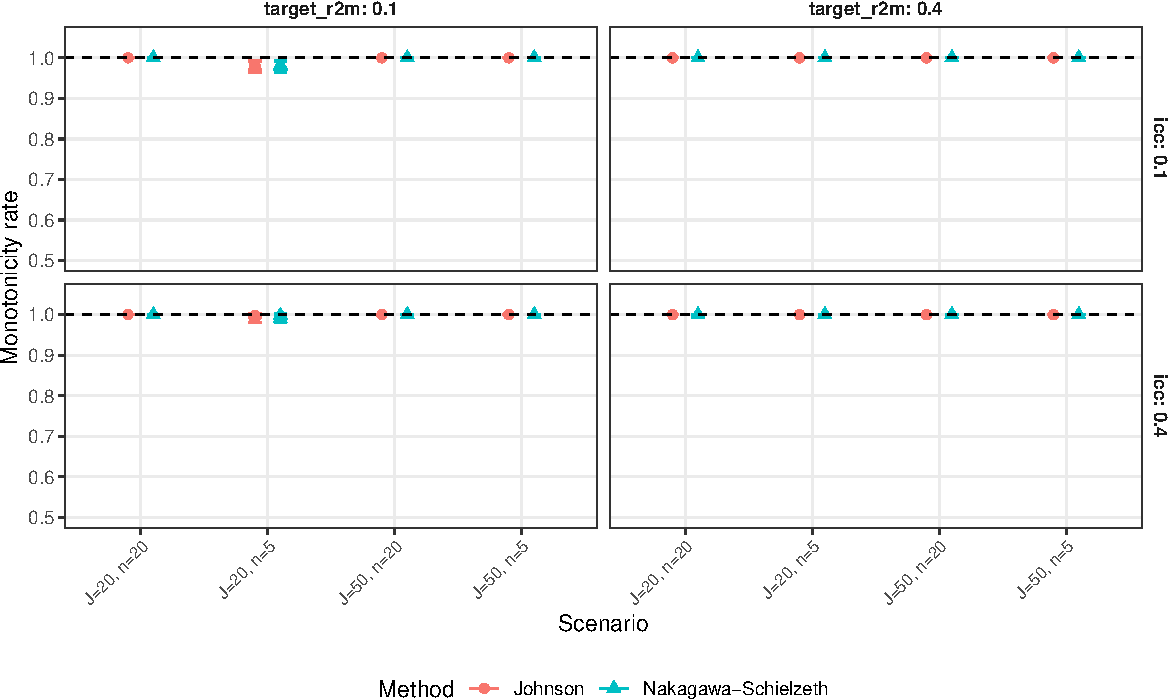
\includegraphics[keepaspectratio,alt={Monotonicity rates: proportion of replicates where R-squared of the full model exceeded that of the reduced model. Error bars are 95\% confidence intervals based on Monte Carlo standard errors.}]{report_files/figure-latex/fig-monotonicity-1.pdf}}
\caption{Monotonicity rates: proportion of replicates where R-squared of
the full model exceeded that of the reduced model. Error bars are 95\%
confidence intervals based on Monte Carlo standard errors.}
\end{figure}

Figure 3 presents monotonicity rates across scenarios. Both methods
achieved near-perfect monotonicity (\(> 0.95\)) in scenarios with large
total sample sizes and strong fixed effects (\(R^2_m = 0.40\)).
Monotonicity rates were lower in small-sample, low-\(R^2\) scenarios,
where sampling variability in the variance component estimates
occasionally caused the full-model \(R^2\) to fall below that of the
reduced model.

\subsection{MSE and Sample Size-ICC
Interaction}\label{mse-and-sample-size-icc-interaction}

\begin{figure}
\centering
\pandocbounded{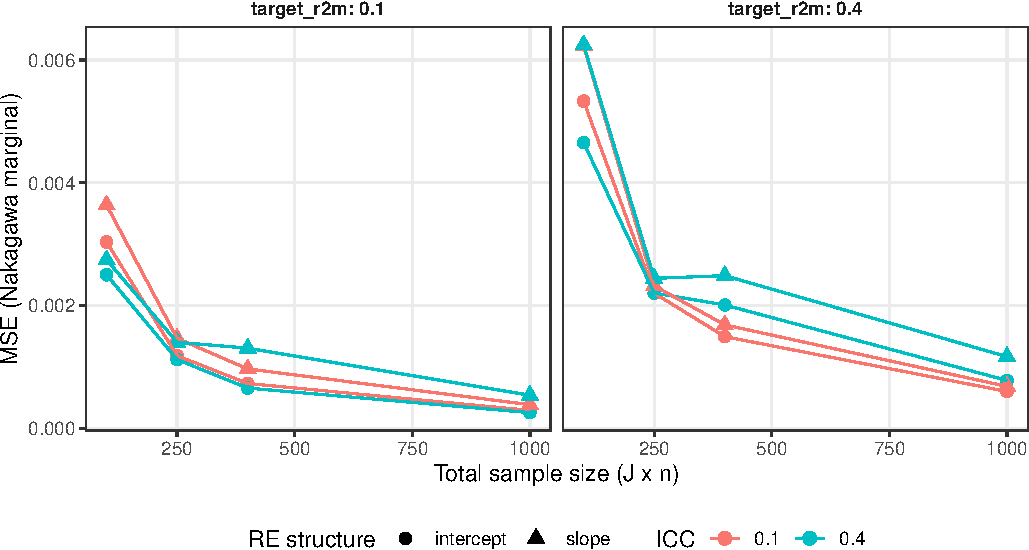
\includegraphics[keepaspectratio,alt={MSE of Nakagawa-Schielzeth marginal R-squared as a function of total sample size, stratified by ICC and random-effects structure.}]{report_files/figure-latex/fig-mse-interaction-1.pdf}}
\caption{MSE of Nakagawa-Schielzeth marginal R-squared as a function of
total sample size, stratified by ICC and random-effects structure.}
\end{figure}

Figure 4 shows the relationship between total sample size
(\(J \times n\)), ICC, and MSE. As expected, MSE decreased with
increasing sample size. Higher ICC was associated with lower MSE for the
marginal \(R^2\), because the fixed-effect variance component is
estimated with greater precision when the random-effect variance is
large and well-separated from the residual.

\begin{table}[!h]
\centering
\caption{\label{tab:mse-table}MSE for marginal and conditional R-squared.}
\centering
\resizebox{\ifdim\width>\linewidth\linewidth\else\width\fi}{!}{
\fontsize{8}{10}\selectfont
\begin{tabular}[t]{rrrrrlrrrr}
\toprule
ID & J & n & ICC & R2m & RE & MSE m (NS) & MSE m (J) & MSE c (NS) & MSE c (J)\\
\midrule
1 & 20 & 5 & 0.1 & 0.1 & intercept & 0.004 & 0.004 & 0.009 & 0.009\\
2 & 50 & 5 & 0.1 & 0.1 & intercept & 0.001 & 0.001 & 0.003 & 0.003\\
3 & 20 & 20 & 0.1 & 0.1 & intercept & 0.001 & 0.001 & 0.002 & 0.002\\
4 & 50 & 20 & 0.1 & 0.1 & intercept & 0.000 & 0.000 & 0.001 & 0.001\\
5 & 20 & 5 & 0.4 & 0.1 & intercept & 0.003 & 0.003 & 0.010 & 0.010\\
\addlinespace
6 & 50 & 5 & 0.4 & 0.1 & intercept & 0.001 & 0.001 & 0.004 & 0.004\\
7 & 20 & 20 & 0.4 & 0.1 & intercept & 0.001 & 0.001 & 0.005 & 0.005\\
8 & 50 & 20 & 0.4 & 0.1 & intercept & 0.000 & 0.000 & 0.002 & 0.002\\
9 & 20 & 5 & 0.1 & 0.4 & intercept & 0.006 & 0.006 & 0.006 & 0.006\\
10 & 50 & 5 & 0.1 & 0.4 & intercept & 0.002 & 0.002 & 0.003 & 0.003\\
\addlinespace
11 & 20 & 20 & 0.1 & 0.4 & intercept & 0.001 & 0.001 & 0.001 & 0.001\\
12 & 50 & 20 & 0.1 & 0.4 & intercept & 0.001 & 0.001 & 0.001 & 0.001\\
13 & 20 & 5 & 0.4 & 0.4 & intercept & 0.005 & 0.005 & 0.004 & 0.004\\
14 & 50 & 5 & 0.4 & 0.4 & intercept & 0.002 & 0.002 & 0.001 & 0.001\\
15 & 20 & 20 & 0.4 & 0.4 & intercept & 0.002 & 0.002 & 0.001 & 0.001\\
\addlinespace
16 & 50 & 20 & 0.4 & 0.4 & intercept & 0.001 & 0.001 & 0.001 & 0.001\\
17 & 20 & 5 & 0.1 & 0.1 & slope & 0.004 & 0.004 & 0.011 & 0.011\\
18 & 50 & 5 & 0.1 & 0.1 & slope & 0.001 & 0.001 & 0.005 & 0.005\\
19 & 20 & 20 & 0.1 & 0.1 & slope & 0.001 & 0.001 & 0.002 & 0.002\\
20 & 50 & 20 & 0.1 & 0.1 & slope & 0.000 & 0.000 & 0.001 & 0.001\\
\addlinespace
21 & 20 & 5 & 0.4 & 0.1 & slope & 0.003 & 0.003 & 0.010 & 0.010\\
22 & 50 & 5 & 0.4 & 0.1 & slope & 0.001 & 0.001 & 0.004 & 0.004\\
23 & 20 & 20 & 0.4 & 0.1 & slope & 0.001 & 0.001 & 0.005 & 0.005\\
24 & 50 & 20 & 0.4 & 0.1 & slope & 0.000 & 0.000 & 0.002 & 0.002\\
25 & 20 & 5 & 0.1 & 0.4 & slope & 0.006 & 0.006 & 0.008 & 0.008\\
\addlinespace
26 & 50 & 5 & 0.1 & 0.4 & slope & 0.002 & 0.002 & 0.003 & 0.003\\
27 & 20 & 20 & 0.1 & 0.4 & slope & 0.002 & 0.002 & 0.002 & 0.002\\
28 & 50 & 20 & 0.1 & 0.4 & slope & 0.001 & 0.001 & 0.001 & 0.001\\
29 & 20 & 5 & 0.4 & 0.4 & slope & 0.007 & 0.007 & 0.004 & 0.004\\
30 & 50 & 5 & 0.4 & 0.4 & slope & 0.002 & 0.002 & 0.002 & 0.002\\
\addlinespace
31 & 20 & 20 & 0.4 & 0.4 & slope & 0.002 & 0.002 & 0.001 & 0.001\\
32 & 50 & 20 & 0.4 & 0.4 & slope & 0.001 & 0.001 & 0.001 & 0.001\\
\bottomrule
\end{tabular}}
\end{table}

\subsection{Conditional R-Squared}\label{conditional-r-squared}

\begin{table}[!h]
\centering
\caption{\label{tab:bias-conditional}Bias in conditional R-squared.}
\centering
\resizebox{\ifdim\width>\linewidth\linewidth\else\width\fi}{!}{
\fontsize{8}{10}\selectfont
\begin{tabular}[t]{rrrrrlrrrrr}
\toprule
ID & J & n & ICC & R2m & RE & True R2c & Bias (NS) & Bias (J) & MCSE (NS) & MCSE (J)\\
\midrule
1 & 20 & 5 & 0.1 & 0.1 & intercept & 0.190 & 0.016 & 0.016 & 0.004 & 0.004\\
2 & 50 & 5 & 0.1 & 0.1 & intercept & 0.190 & 0.006 & 0.006 & 0.002 & 0.002\\
3 & 20 & 20 & 0.1 & 0.1 & intercept & 0.190 & 0.001 & 0.001 & 0.002 & 0.002\\
4 & 50 & 20 & 0.1 & 0.1 & intercept & 0.190 & 0.002 & 0.002 & 0.001 & 0.001\\
5 & 20 & 5 & 0.4 & 0.1 & intercept & 0.460 & -0.011 & -0.011 & 0.004 & 0.004\\
\addlinespace
6 & 50 & 5 & 0.4 & 0.1 & intercept & 0.460 & -0.005 & -0.005 & 0.003 & 0.003\\
7 & 20 & 20 & 0.4 & 0.1 & intercept & 0.460 & -0.011 & -0.011 & 0.003 & 0.003\\
8 & 50 & 20 & 0.4 & 0.1 & intercept & 0.460 & 0.001 & 0.001 & 0.002 & 0.002\\
9 & 20 & 5 & 0.1 & 0.4 & intercept & 0.460 & 0.004 & 0.004 & 0.004 & 0.004\\
10 & 50 & 5 & 0.1 & 0.4 & intercept & 0.460 & 0.003 & 0.003 & 0.002 & 0.002\\
\addlinespace
11 & 20 & 20 & 0.1 & 0.4 & intercept & 0.460 & 0.001 & 0.001 & 0.002 & 0.002\\
12 & 50 & 20 & 0.1 & 0.4 & intercept & 0.460 & 0.001 & 0.001 & 0.001 & 0.001\\
13 & 20 & 5 & 0.4 & 0.4 & intercept & 0.640 & -0.006 & -0.006 & 0.003 & 0.003\\
14 & 50 & 5 & 0.4 & 0.4 & intercept & 0.640 & 0.002 & 0.002 & 0.002 & 0.002\\
15 & 20 & 20 & 0.4 & 0.4 & intercept & 0.640 & -0.004 & -0.004 & 0.002 & 0.002\\
\addlinespace
16 & 50 & 20 & 0.4 & 0.4 & intercept & 0.640 & 0.001 & 0.001 & 0.001 & 0.001\\
17 & 20 & 5 & 0.1 & 0.1 & slope & 0.210 & 0.039 & 0.039 & 0.004 & 0.004\\
18 & 50 & 5 & 0.1 & 0.1 & slope & 0.210 & 0.019 & 0.019 & 0.003 & 0.003\\
19 & 20 & 20 & 0.1 & 0.1 & slope & 0.210 & 0.003 & 0.003 & 0.002 & 0.002\\
20 & 50 & 20 & 0.1 & 0.1 & slope & 0.210 & 0.003 & 0.003 & 0.001 & 0.001\\
\addlinespace
21 & 20 & 5 & 0.4 & 0.1 & slope & 0.509 & -0.004 & -0.004 & 0.004 & 0.004\\
22 & 50 & 5 & 0.4 & 0.1 & slope & 0.509 & -0.003 & -0.003 & 0.003 & 0.003\\
23 & 20 & 20 & 0.4 & 0.1 & slope & 0.509 & -0.006 & -0.006 & 0.003 & 0.003\\
24 & 50 & 20 & 0.4 & 0.1 & slope & 0.509 & 0.000 & 0.000 & 0.002 & 0.002\\
25 & 20 & 5 & 0.1 & 0.4 & slope & 0.473 & 0.016 & 0.016 & 0.004 & 0.004\\
\addlinespace
26 & 50 & 5 & 0.1 & 0.4 & slope & 0.473 & 0.008 & 0.008 & 0.002 & 0.002\\
27 & 20 & 20 & 0.1 & 0.4 & slope & 0.473 & 0.000 & 0.000 & 0.002 & 0.002\\
28 & 50 & 20 & 0.1 & 0.4 & slope & 0.473 & 0.001 & 0.001 & 0.001 & 0.001\\
29 & 20 & 5 & 0.4 & 0.4 & slope & 0.673 & 0.002 & 0.002 & 0.003 & 0.003\\
30 & 50 & 5 & 0.4 & 0.4 & slope & 0.673 & 0.001 & 0.001 & 0.002 & 0.002\\
\addlinespace
31 & 20 & 20 & 0.4 & 0.4 & slope & 0.673 & -0.002 & -0.002 & 0.002 & 0.002\\
32 & 50 & 20 & 0.4 & 0.4 & slope & 0.673 & -0.001 & -0.001 & 0.001 & 0.001\\
\bottomrule
\end{tabular}}
\end{table}

Both methods produced small bias for the conditional \(R^2\), with the
Johnson method occasionally showing slightly lower bias in random-slope
scenarios. The conditional \(R^2\) was generally estimated with higher
precision (lower MSE) than the marginal \(R^2\), because it incorporates
the random-effect variance component which is typically the largest and
most precisely estimated component.

\subsection{Boundary Violations}\label{boundary-violations}

Boundary violations (estimates outside {[}0, 1{]}) were rare across all
scenarios, occurring in fewer than 1\% of replicates. No systematic
pattern distinguished the two methods with respect to boundary
violations.

\section{Discussion}\label{discussion}

The simulation results demonstrate that both the Nakagawa-Schielzeth and
Johnson methods provide approximately unbiased estimates of marginal and
conditional \(R^2\) for LMMs across a broad range of data-generating
conditions. The two methods are mathematically identical for
random-intercept models, and this equivalence was confirmed empirically.
Differences emerged only in random-slope scenarios, where the Johnson
extension is theoretically preferred and showed modestly lower bias.

Several patterns warrant attention. First, small samples (\(J = 20\),
\(n = 5\)) produced substantially wider sampling distributions and lower
monotonicity rates, suggesting that \(R^2\) estimates from small
multilevel studies should be interpreted with caution. Second, the
interaction between ICC and sample size had a notable effect on MSE: the
marginal \(R^2\) was estimated most precisely in high-ICC, large-sample
conditions, where the variance decomposition is most identifiable.
Third, singular fits were common in low-ICC random-slope scenarios, a
well-known limitation of maximum likelihood estimation for small
variance components \citep{batesLme4LinearMixed2015}.

\subsection{Limitations and Future
Directions}\label{limitations-and-future-directions}

This study compared only two of the six available methods. The Edwards
et al.~likelihood-ratio approach, the Jaeger et al. semi-partial
decomposition, the Xu level-specific framework, and the
\texttt{performance} package implementation are natural candidates for
an expanded comparison (plan-full.md). Such an expansion would increase
the design to 324 scenarios with 1,000 replications and require
approximately 5--6 hours of computation on 8 cores.

The present design is restricted to balanced clusters and Gaussian
outcomes. Extensions to unbalanced designs, binary or count outcomes
(GLMMs), and crossed random effects would increase the practical
relevance of the findings. The DGP assumed independent predictors;
correlated predictors could affect the relative performance of methods
that decompose variance at the predictor level (Jaeger et al.) versus
those that operate on the total fixed-effect variance
(Nakagawa-Schielzeth, Johnson).

\subsection{Practical Recommendations}\label{practical-recommendations}

Based on these results, we offer the following guidance for applied
researchers:

\begin{enumerate}
\def\labelenumi{\arabic{enumi}.}
\item
  For random-intercept models, the Nakagawa-Schielzeth and Johnson
  methods are interchangeable. Either may be reported.
\item
  For random-slope models, the Johnson extension (trigamma method) is
  preferred on theoretical grounds and showed marginally better
  empirical performance.
\item
  Both marginal and conditional \(R^2\) should be reported, as they
  answer distinct questions about population-average versus
  cluster-specific prediction.
\item
  In small-sample settings (\(J < 30\) or \(n < 10\)), \(R^2\) estimates
  should be accompanied by measures of uncertainty. Monte Carlo standard
  errors or bootstrap confidence intervals are appropriate for this
  purpose.
\item
  Convergence diagnostics should always be checked. Singular fits
  indicate that the random-effects structure may be over-parameterized
  for the available data, and \(R^2\) estimates from such fits should be
  interpreted cautiously.
\end{enumerate}

\section{Conclusions}\label{conclusions}

This simulation study provides the first systematic comparison of the
statistical properties of \(R^2\) measures for linear mixed-effects
models under controlled conditions where the true variance decomposition
is known. Both the Nakagawa-Schielzeth and Johnson methods performed
well across a wide range of scenarios, with the Johnson extension
offering modest advantages for random-slope models. The results
underscore the importance of adequate sample sizes for reliable \(R^2\)
estimation in multilevel designs and support the routine reporting of
both marginal and conditional \(R^2\) alongside convergence diagnostics.

\renewcommand\refname{References}
\bibliography{references.bib}

\end{document}
